% Appendices are set up same as chapter sections
\chapter{Appendix - Proposed App Interface}

\begin{figure}[h]
  \centering
     \includegraphics[scale=0.75]{images/App_flow.png}
  \caption{App flow we designed in order to implement the smartphone app}
  \label{fig:App_flow}
\end{figure}

\begin{figure}[h]
  \centering
     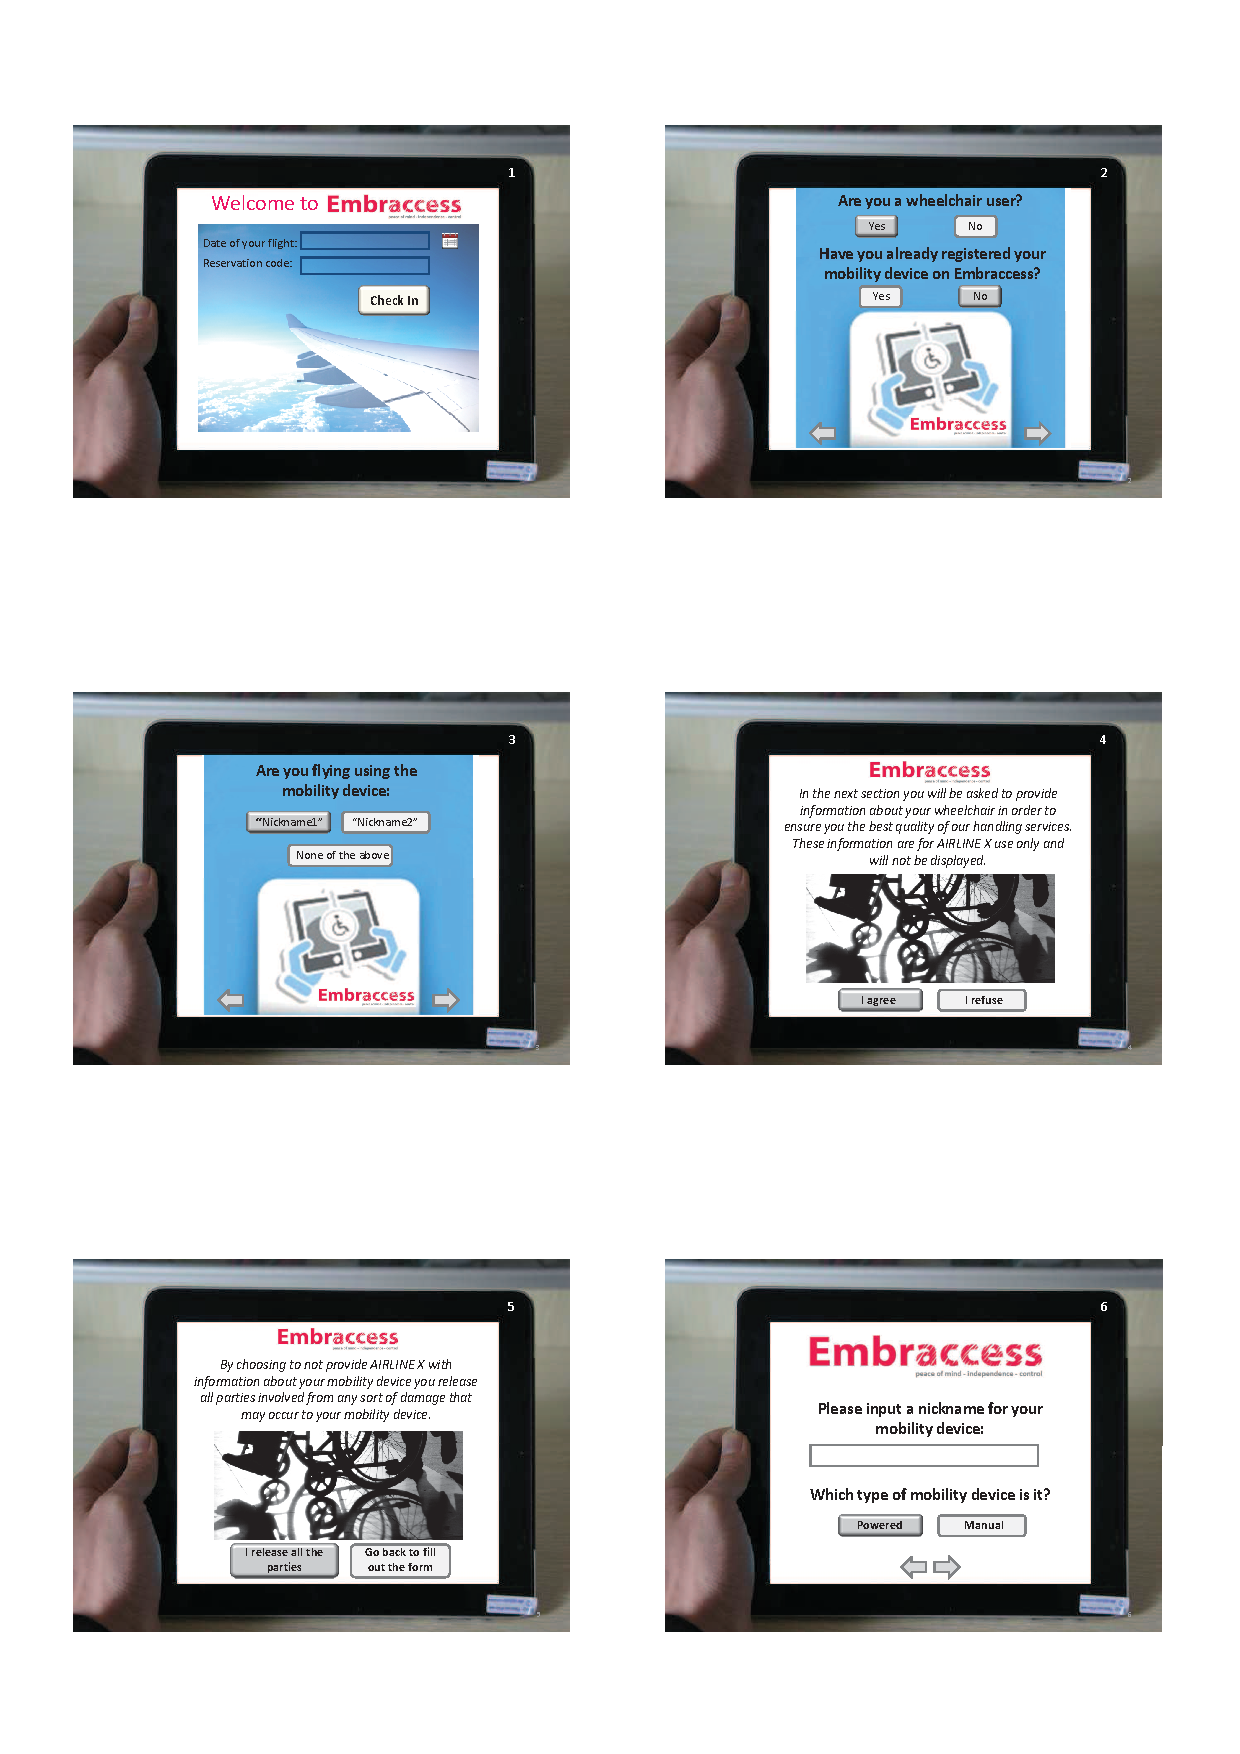
\includegraphics[scale=0.75]{images/App_UI_1.pdf}
  \label{fig:App_UI_1}
\end{figure}

\begin{figure}[h]
  \centering
     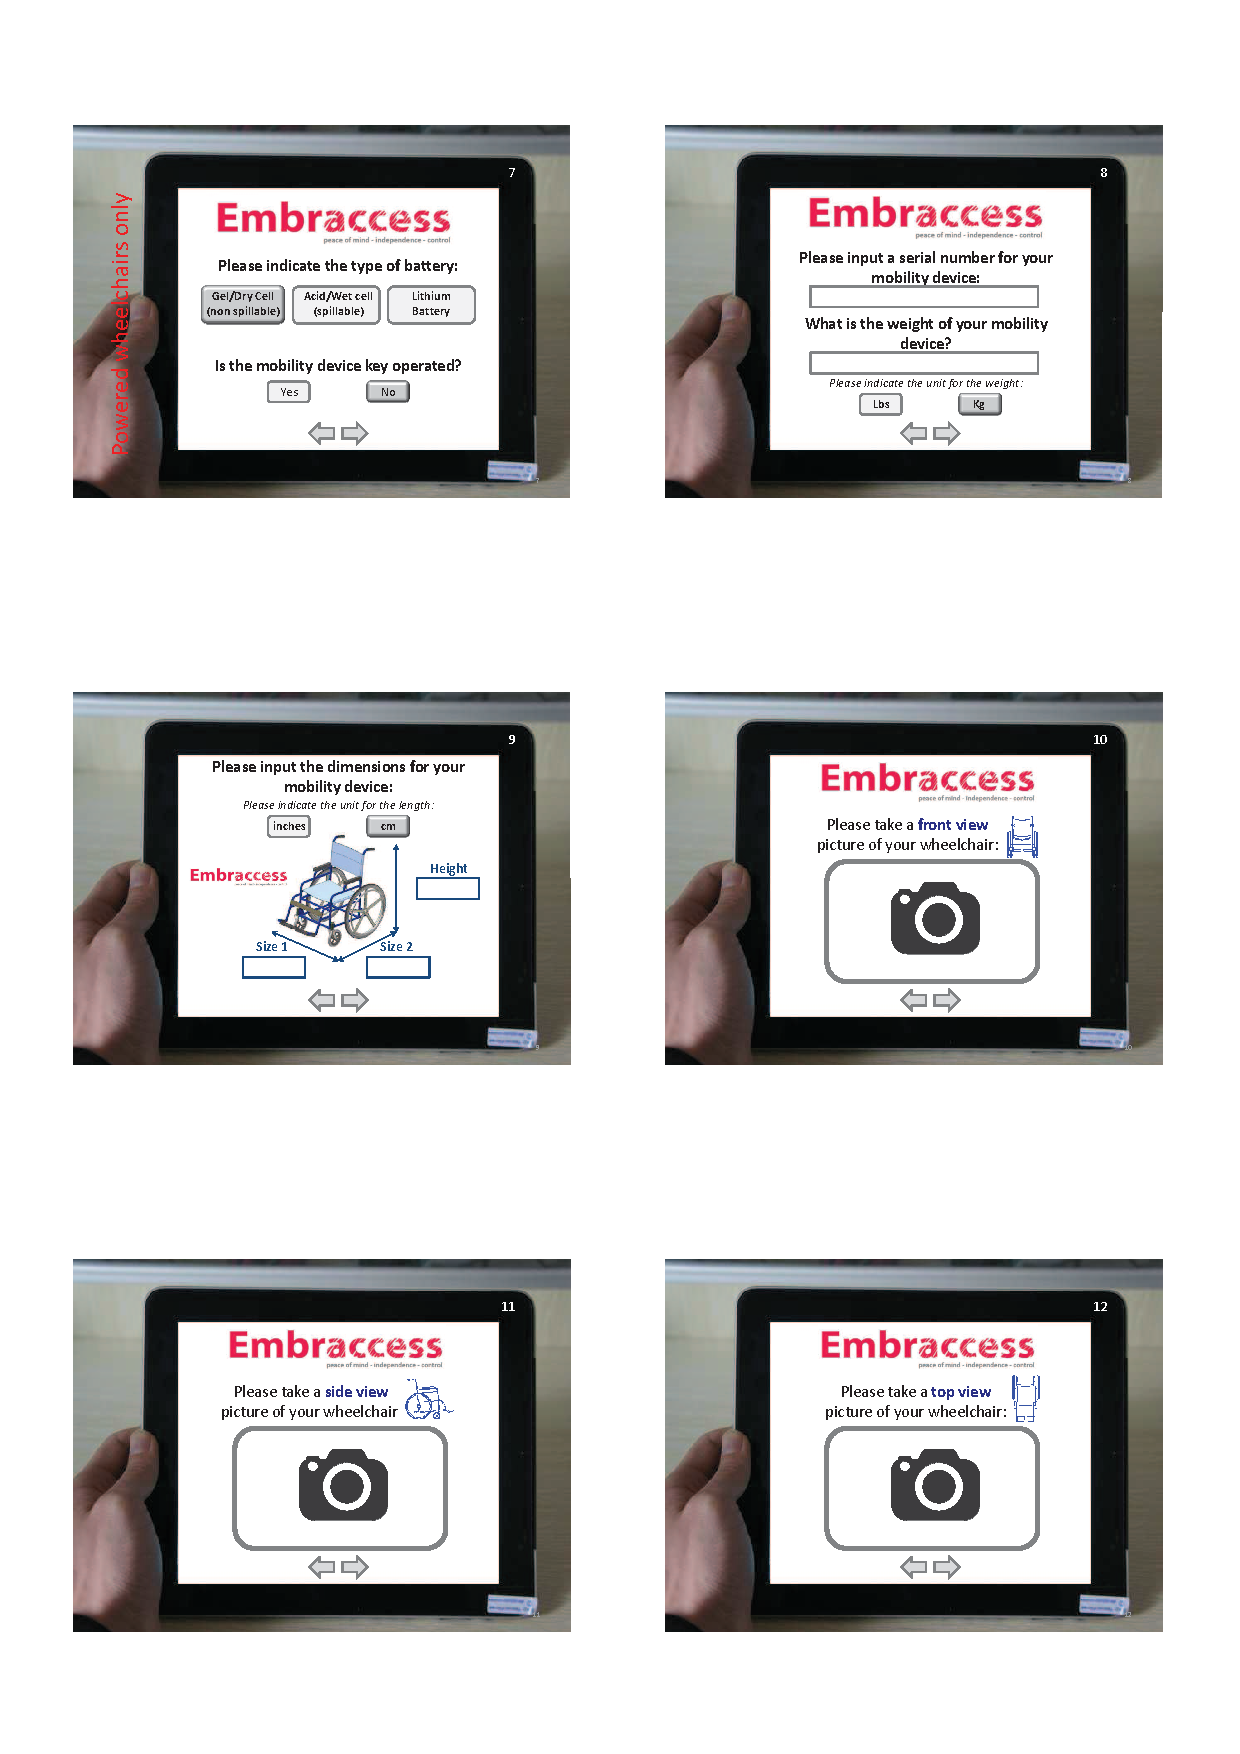
\includegraphics[scale=0.75]{images/App_UI_2.pdf}
  \label{fig:App_UI_2}
\end{figure}

\begin{figure}[h]
  \centering
     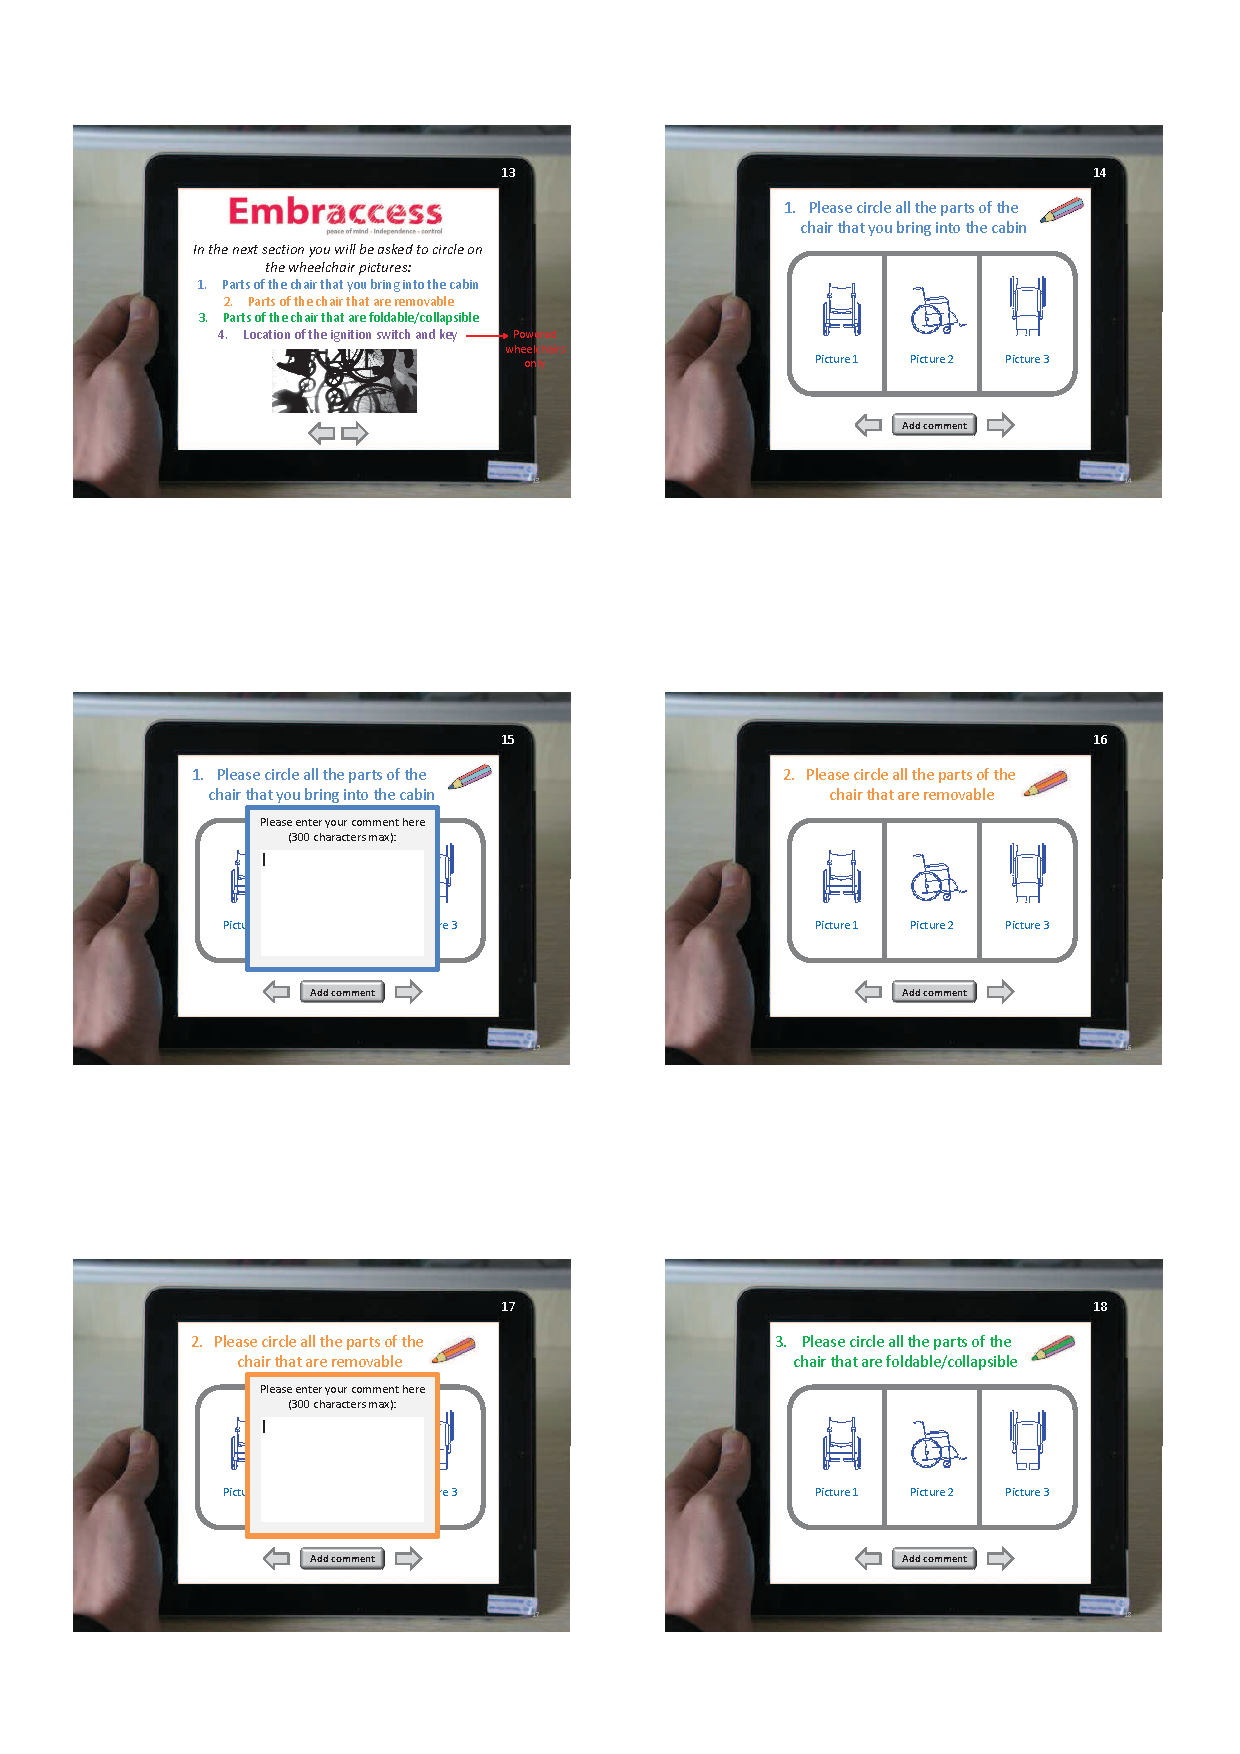
\includegraphics[scale=0.75]{images/App_UI_3.pdf}
  \label{fig:App_UI_3}
\end{figure}

\begin{figure}[h]
  \centering
     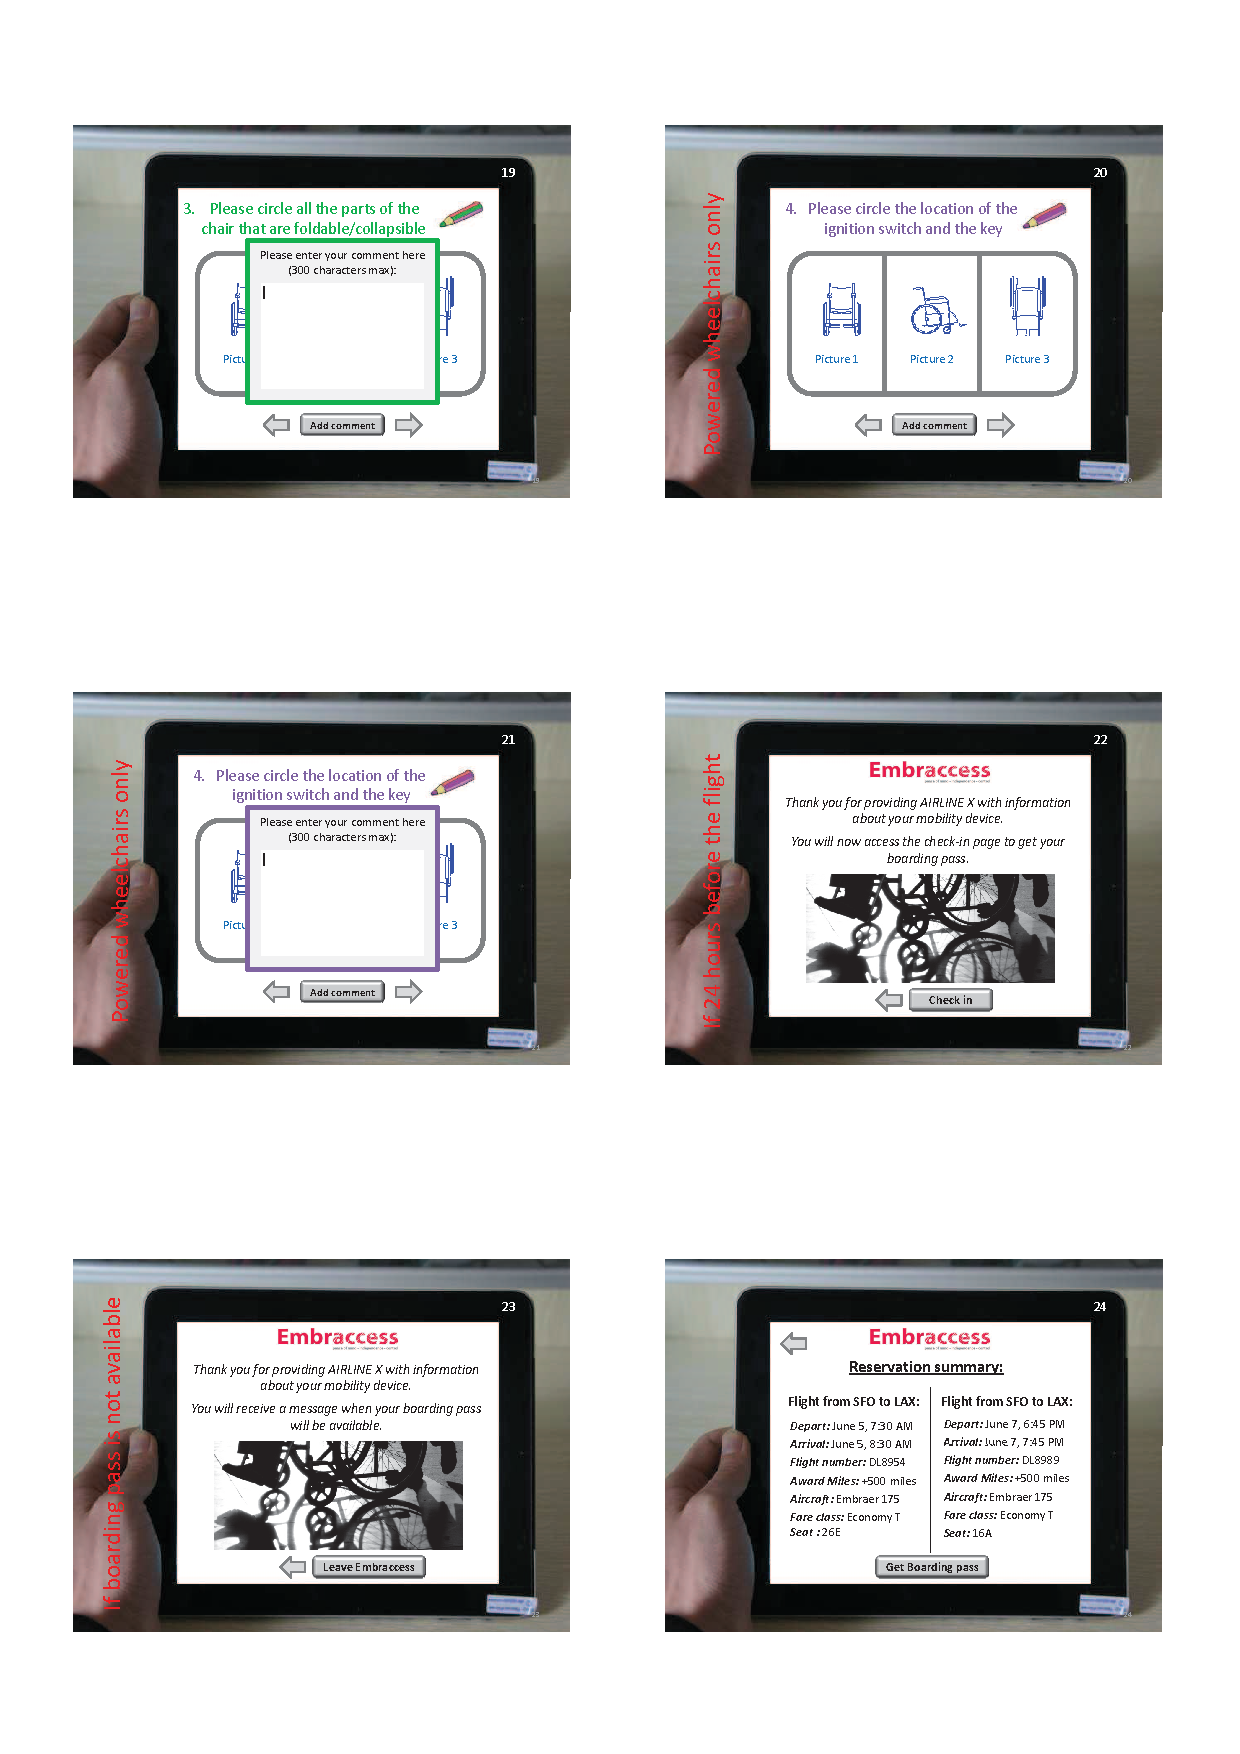
\includegraphics[scale=0.75]{images/App_UI_4.pdf}
  \label{fig:App_UI_4}
\end{figure}

\begin{figure}[h]
  \centering
     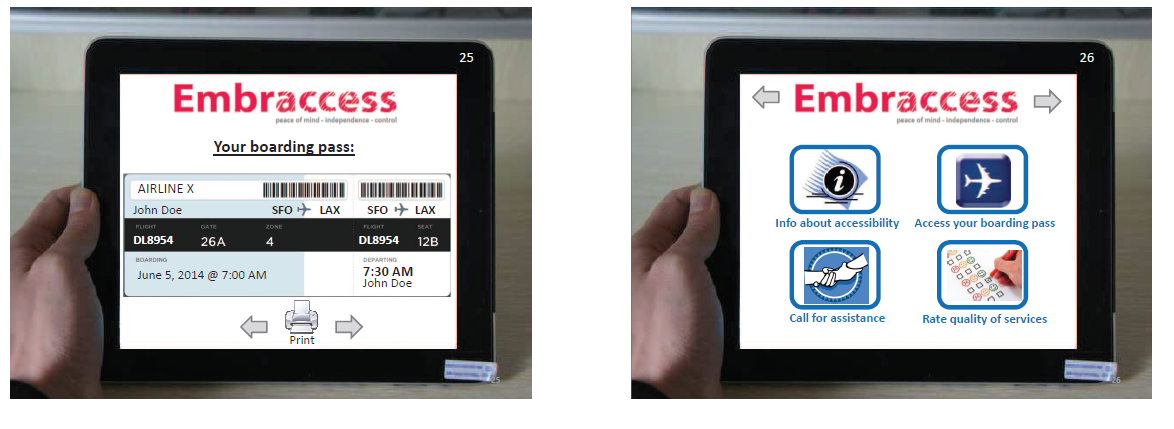
\includegraphics[scale=0.5]{images/App_UI_5.png}
  \caption{App user interface we imagined in order to implement the smartphone app}
  \label{fig:App_UI_5}
\end{figure}

\newpage

Our team thought it would be great if disabled passengers were able to give and receive important information via a smartphone app to make sure their flying experience would not turn out into a nightmare. As shown on the app flow and the user interface we imagined, this app could be integrated to the already existing airline app that enables every single passenger to get their boarding passes.\\

Since airlines do not always anticipate wheelchair users on their regular flight, we designed the app such that any wheelchair user would be strongly encouraged to give information about his situation and his mobility device before getting his boarding pass. This is a way to ensure that airlines are aware in advance of how many disabled passengers will be flying with them and what type of mobility device they will bring.\\

Indeed, we plan on using the smartphone camera to allow people to send pictures of their mobility device. This way, airlines know what to expect at the gate and can make special arrangement with the handlers if needed. Moreover, passengers have the opportunity to write down messages or important precisions on their pictures that will be carefully analyzed by baggage handlers.\\
Once all the information about the mobility device will be provided, users can access their boarding pass if available. After this, the app will offer an interface with four different categories available all along the flying experience:

\begin{itemize}

\item \textbf{Info about accessibility:} this section will locate in which airport and terminal passengers are located and will provide them with information about accessible bathroom, elevator locations, etc.

\item \textbf{Access your boarding pass:} if at any time passengers need to reopen their boarding pass our check information about their reservation, this section will allow them to do so.

\item \textbf{Call for assistance:} if at any time a disabled passenger needs assistance for carrying his luggage, get an airport wheelchair, go through security, etc., this section will enable him to call an airport employee that will come to help him.

\item \textbf{Rate quality f services:} in order to make sure airline services meet disabled passengers’ expectations, the app will allow them to rate the quality of services (pre-boarding, wheelchair handling, transfer to the seat, assistance if using restroom during the flight, etc.)


\end{itemize}
